\section{Model 1: $E_3$}

The results displayed in this section are for the uncertainty involved in the calculation of flamespeed depending only on one parameter i.e the activation energy for the fall off reaction in the ozone mechanism. The percentage of ozone is taken as 40,46,53,75 and 100  percent acccording to the experimental data available to us from Streng\cite{Streng}.The results are displayed in five sections. In first section, the plots are shown for raw chain size, histogram, CDF and log likelihood for parameter $E_3$. In second section, for constant surrogate size, the number of samples are changed from 1e5 to 1e7 and convergence is observed. In the third part of the results, convergence study is done for surrogates with different sizes. In fourth section, we ensure that samples of the parameter which we are drawing are fitting the flamespeed values of the experiment. Also for varying size the map point of the resulting pdf does not change greatly. In the fifth section mean and correlation plots are shown for the samples of the parameter. The surrogates for individual concentrations are constructed using linear interpolation function. The initial guess for the map point is calculated using nelder mead optimization technique. After supplying initial guess over large domain it is found that the map point is the same no matter where we start our guess. 
\bigskip

\subsection{ Statistics }

\noindent In this section, we display results for sample size 1e7 and surrogate of 1000 points. We show the raw samples generated by MCMC and plot the histogram for the same. Later we plot the kde and cdf. The last plot shows the log of the likelihood function. We can clearly see the burning period for the samples. 

\begin{figure}[H]
\centering
\subfloat[MCMC raw chain of samples \label{subfig-1:Raw Chain}]{%
     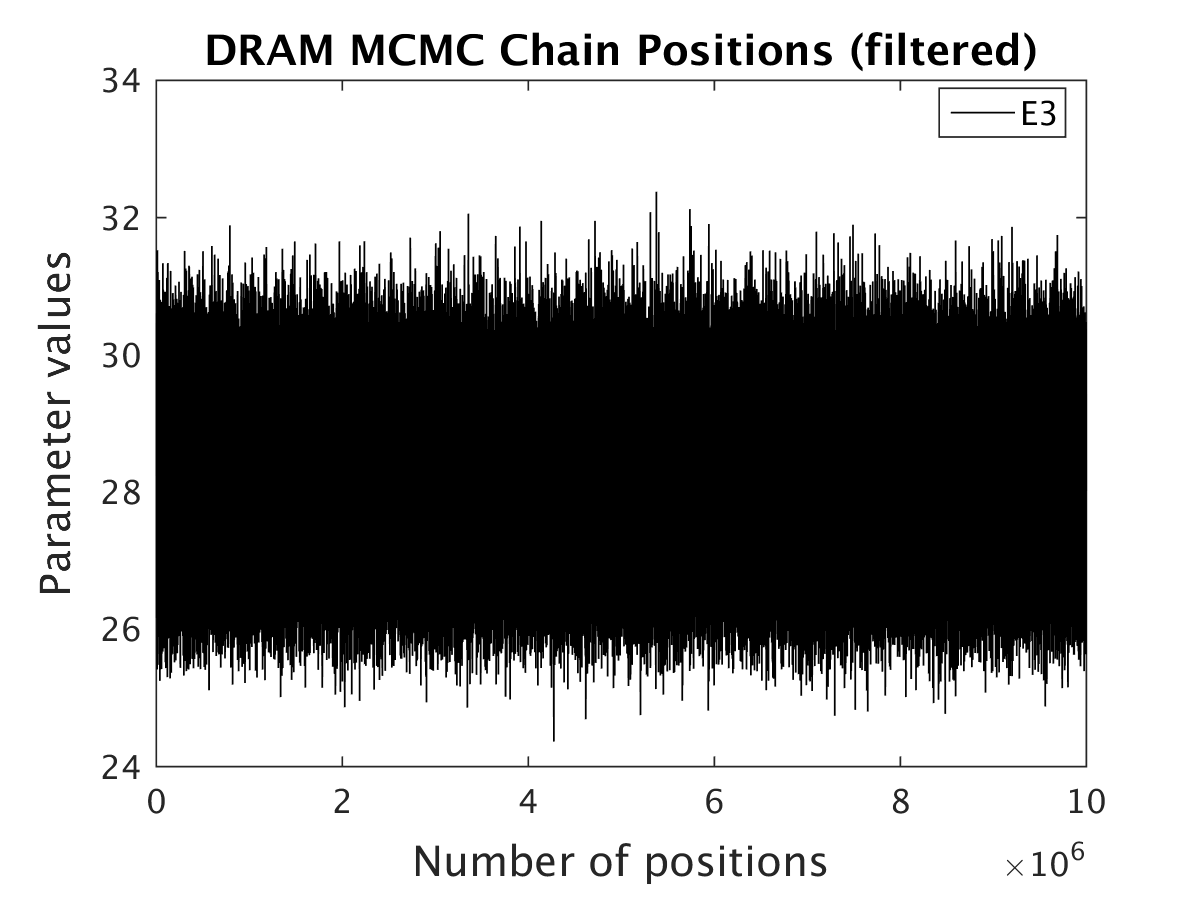
\includegraphics[scale=0.7]{model_1/simple_ip_chain_pos_filt} 
    }
    \quad
\subfloat[Histogram\label{subfig-2:Histogram}]{%
     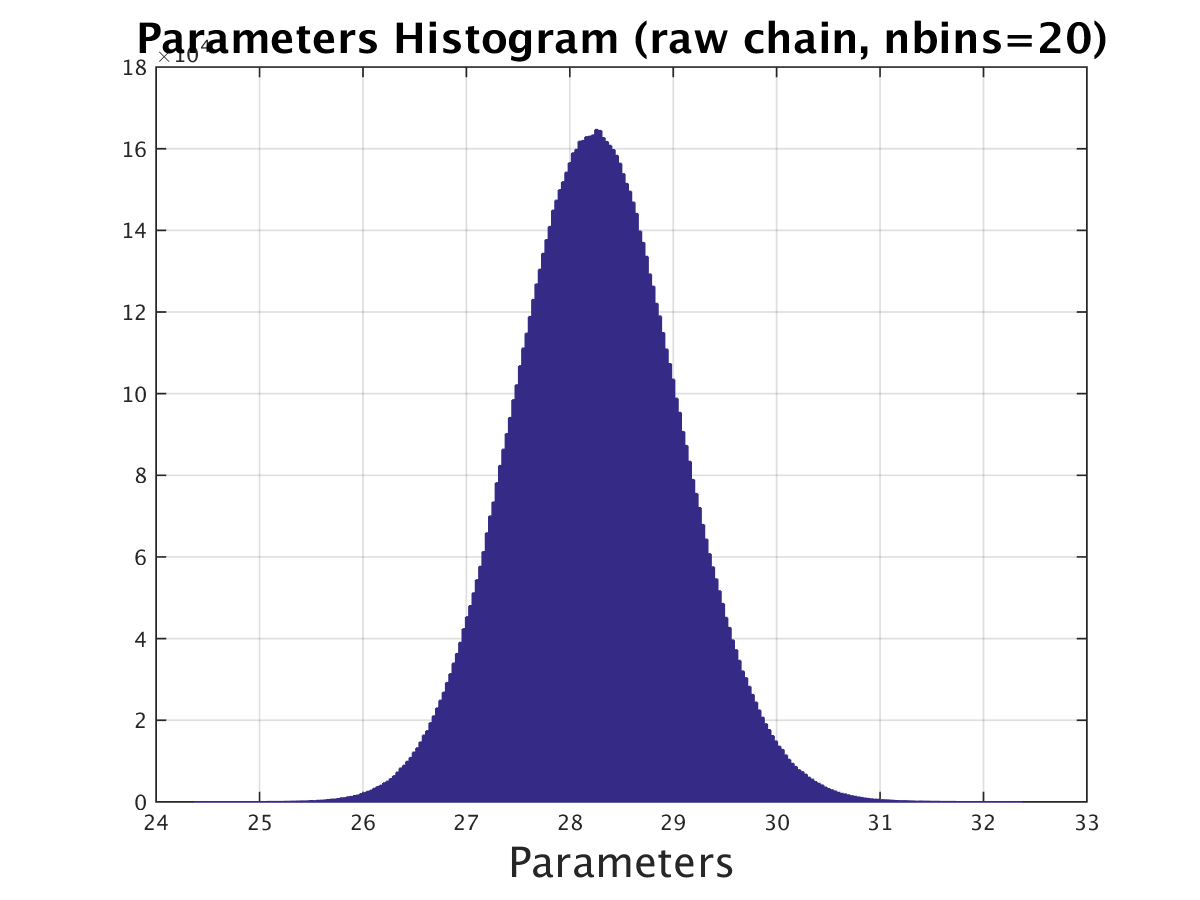
\includegraphics[scale=0.7]{model_1/simple_ip_hist_raw} 
    }
    \end{figure}
  \begin{figure}[H]
  \ContinuedFloat
  \centering
   \subfloat[Cummulative Density Funtion \label{subfig-3:CDF}]{
        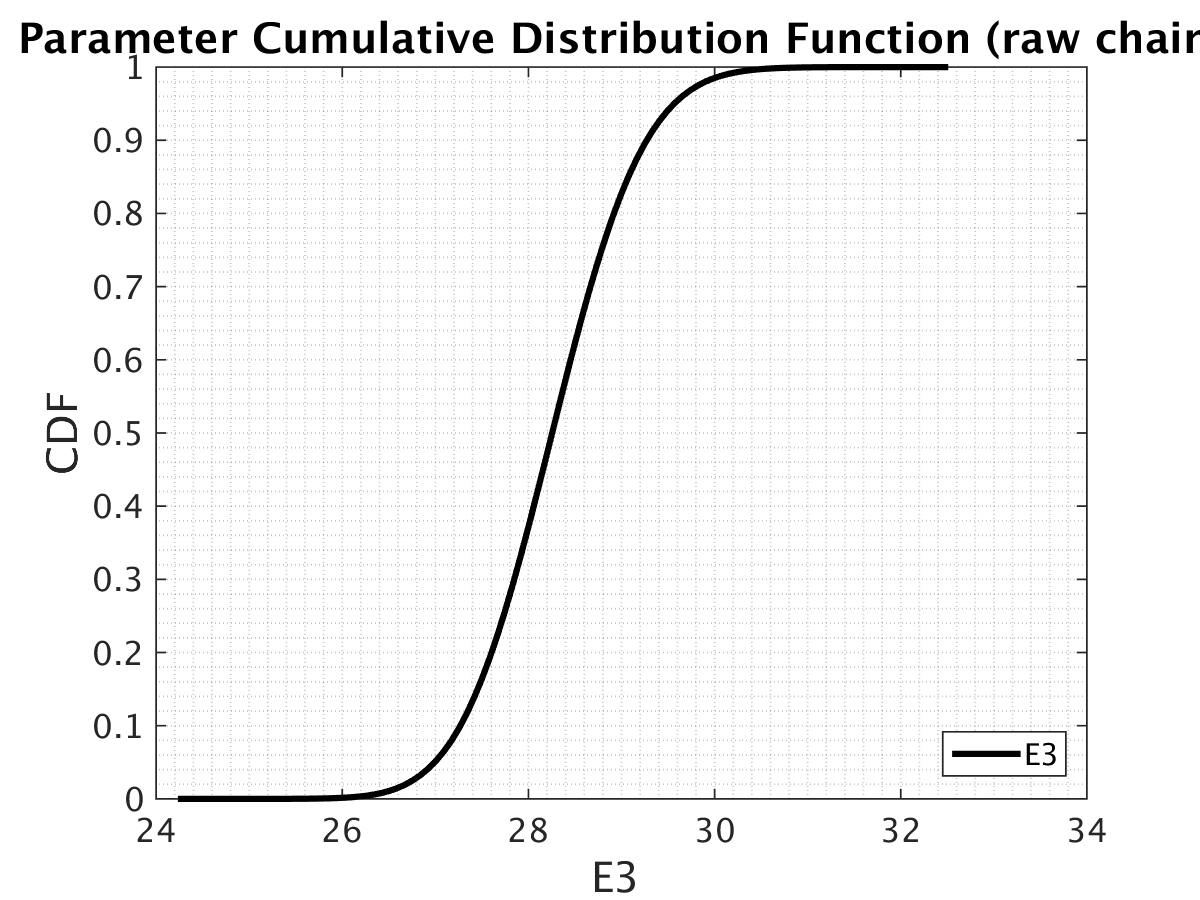
\includegraphics[scale=0.7]{model_1/simple_ip_cdf_raw} 
       }
     \quad
\subfloat[KDE \label{subfig-4:KDE}]{
        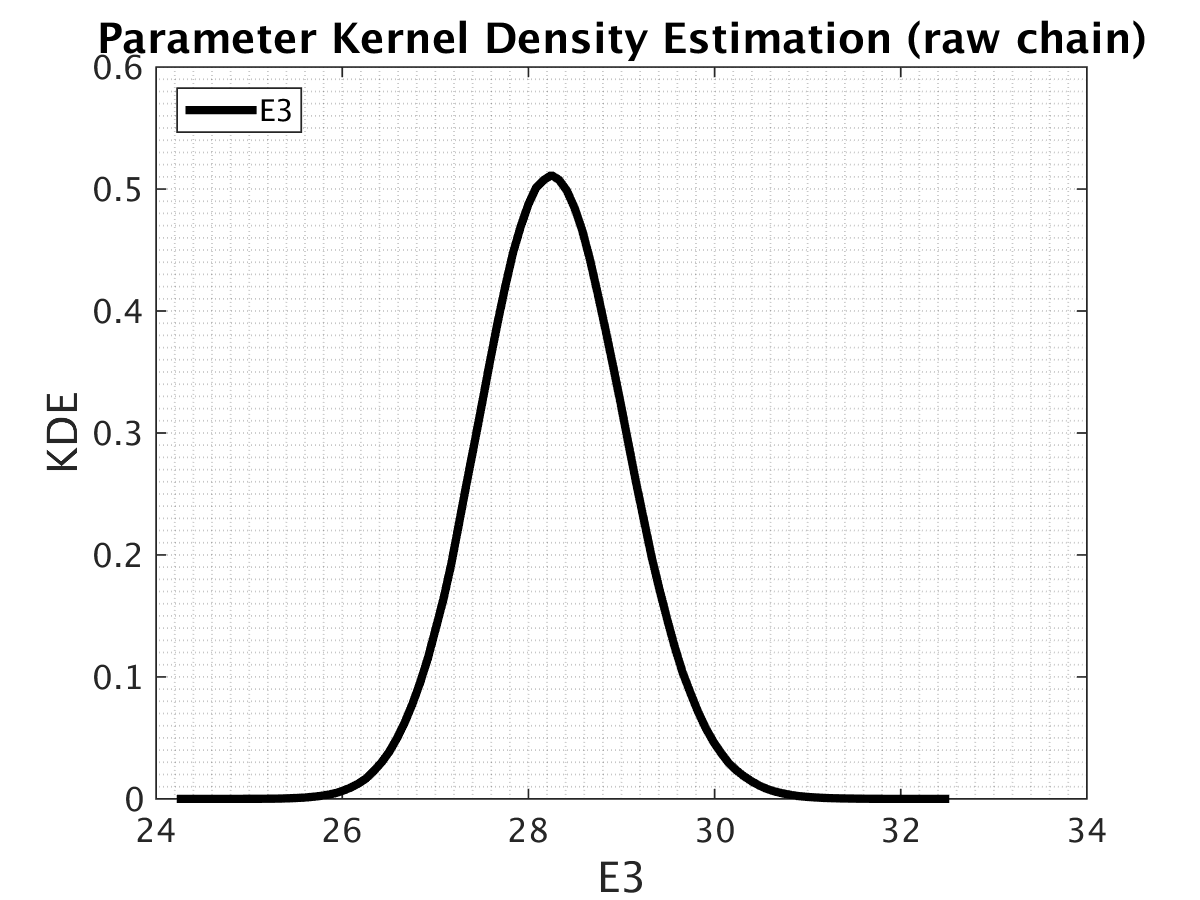
\includegraphics[scale=0.7]{model_1/simple_ip_kde_raw} 
            }  
\end{figure}
\begin{figure}[H]
 \ContinuedFloat
\centering
\subfloat[LogLikelihood \label{subfig-5:Loglike}]{
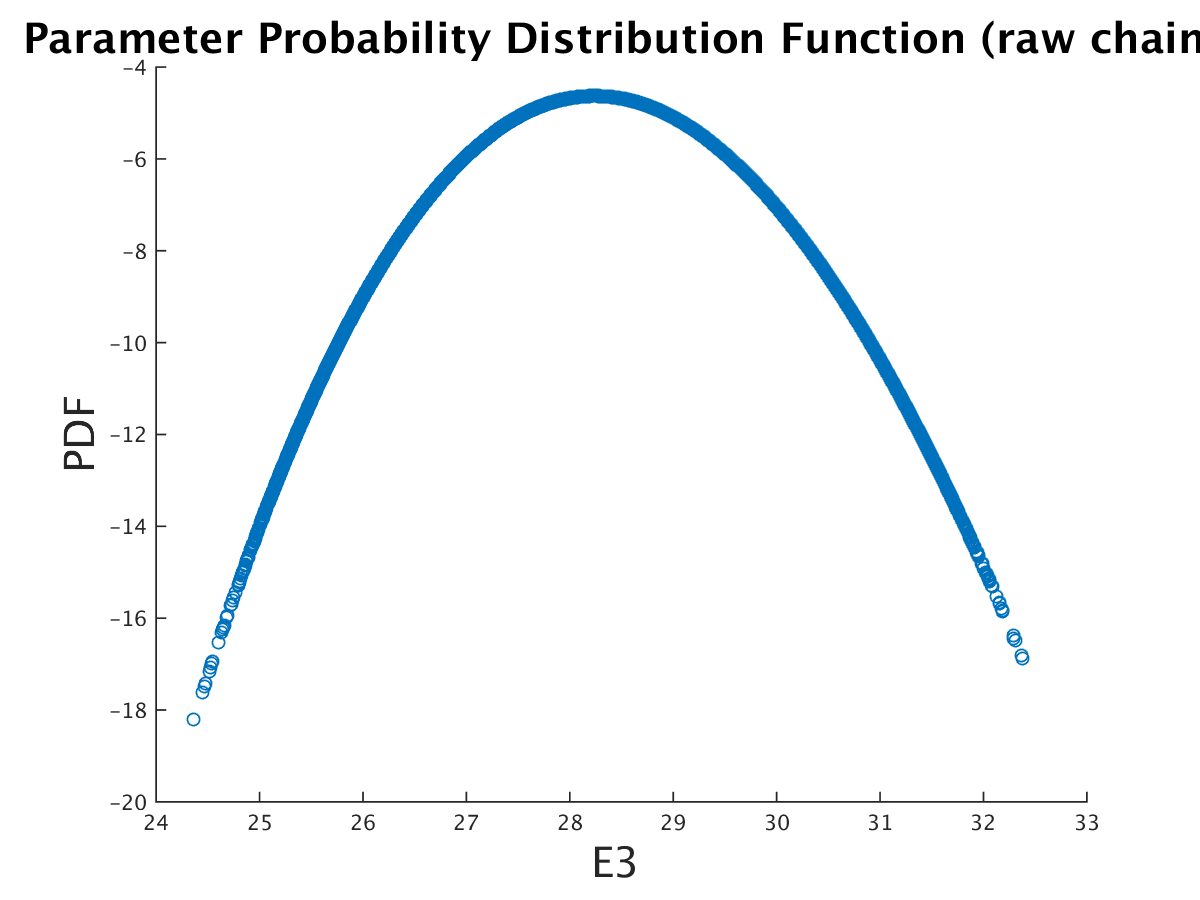
\includegraphics[scale=0.7]{model_1/ip_logLike_unified} 
  }
    \caption{Results for sample size 1e7}
\end{figure}




%\subsection{Convergence Study }
%
%\noindent In this section, we see the convergence of the probability distribution as we increase the raw chain sample size. The plot is done for surrogate size of 1000. In this analysis, raw chain size of $1e5$, $5e5$ , $1e6$, $5e6$ and $1e7$ is taken. 
%
%\begin{figure}[H]
%\centering
%\subfloat[ Convergence  \label{subfig-1:dummy}]{
%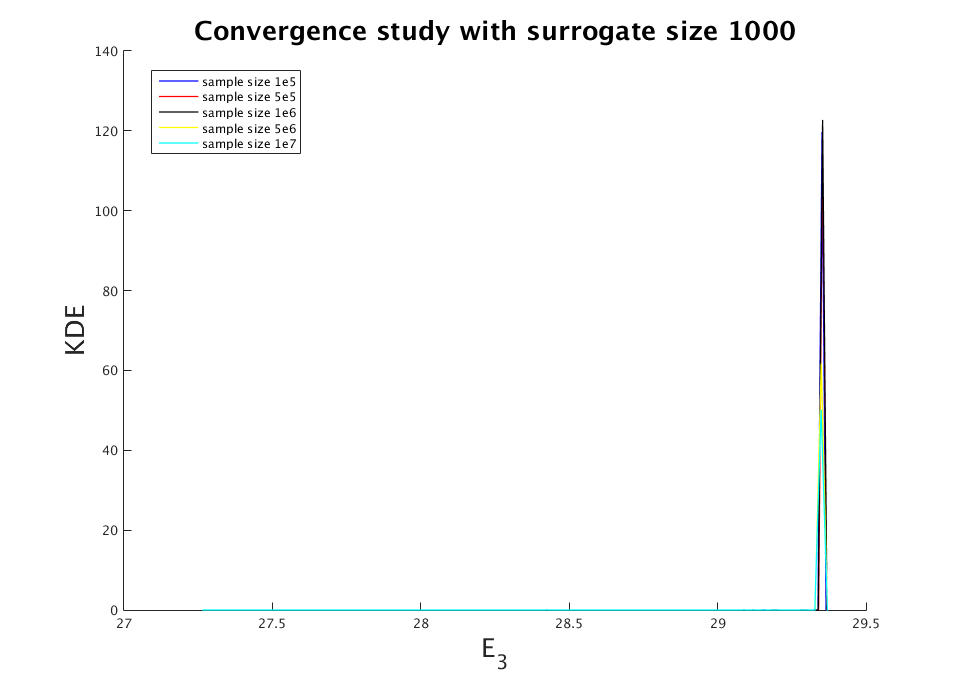
\includegraphics[scale=0.7]{one_parameter/1000_kde/convergence_study/conv} 
%  }
%    \caption{Convergence for surrogate size 1000}
%\end{figure}
%
%
%\subsection{flamespeed Data fit}
%
%\noindent It is necessary to ensure that the samples of the parameter which we are drawing are fitting the flamespeed values of the experiment. In this section, we calculate the flamespeed for all the parameters drawn using the surrogate generated before. We have taken $1e7$ sample size and calculated flamespeed for different concentrations of ozone. 
%
%\begin{figure}[H]
%\centering
%\subfloat[ Flame speed for 20 \% ozone   \label{subfig-1:dummy}]{
%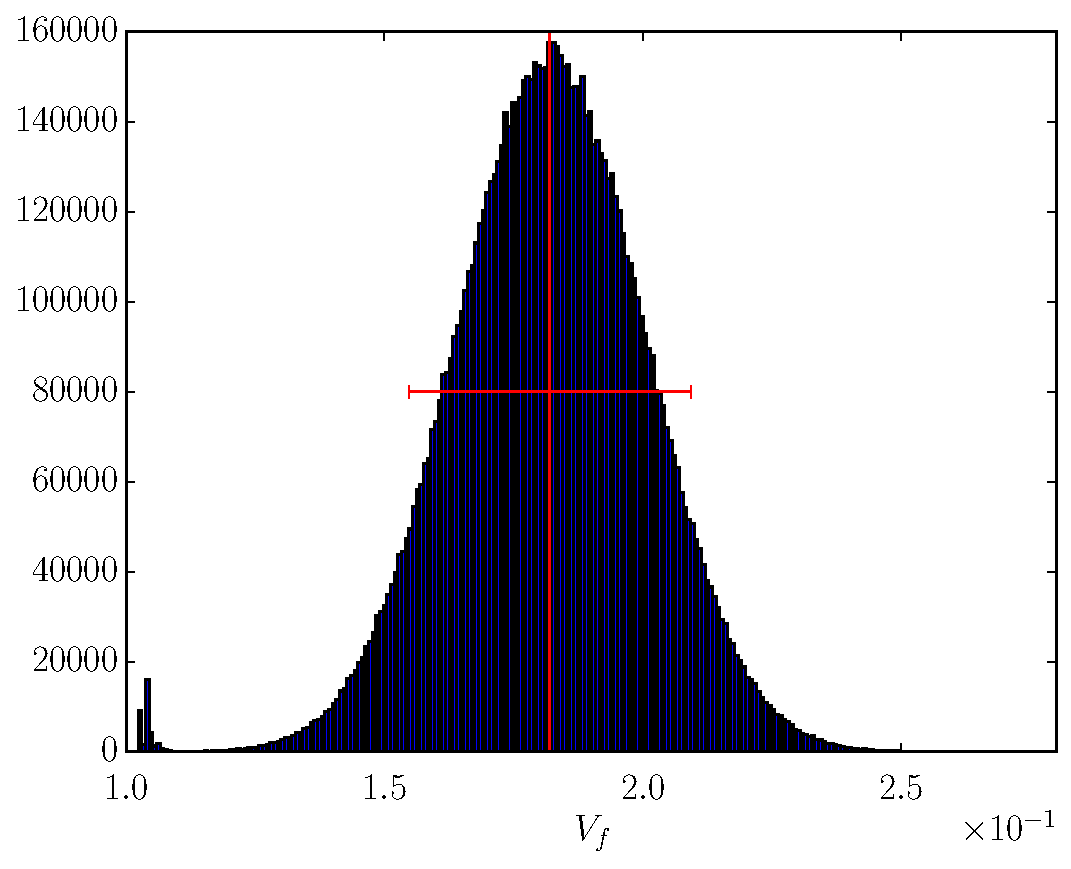
\includegraphics[scale=0.7]{one_parameter/flamespeed_calculation/flame_20.pdf} 
%  }
%  \quad
%  \subfloat[ Flame speed for 28 \% ozone   \label{subfig-1:dummy}]{
%  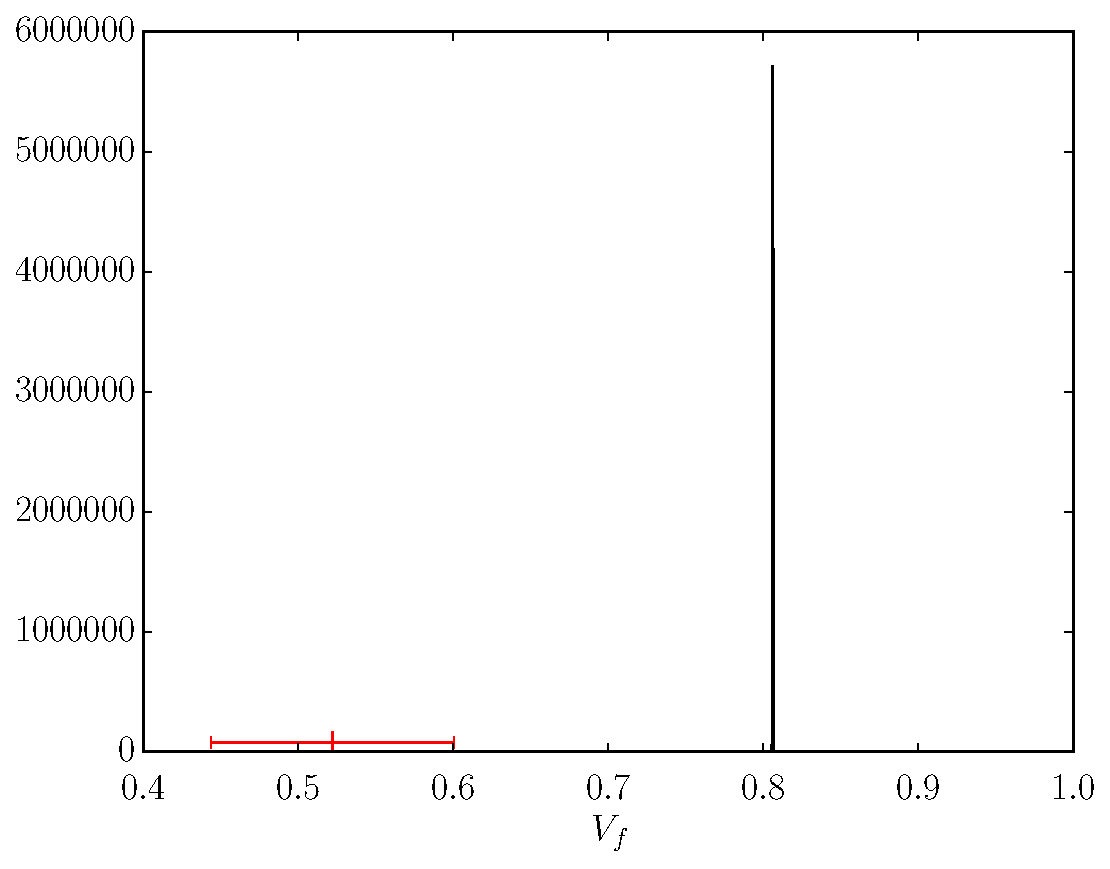
\includegraphics[scale=0.7]{one_parameter/flamespeed_calculation/flame_28.pdf} 
%    }
%\end{figure}
%
%
% \begin{figure}[H]
%  \ContinuedFloat
%  \centering
%   \subfloat[ Flame speed for 40 \% ozone \label{subfig-1:dummy}]{
%        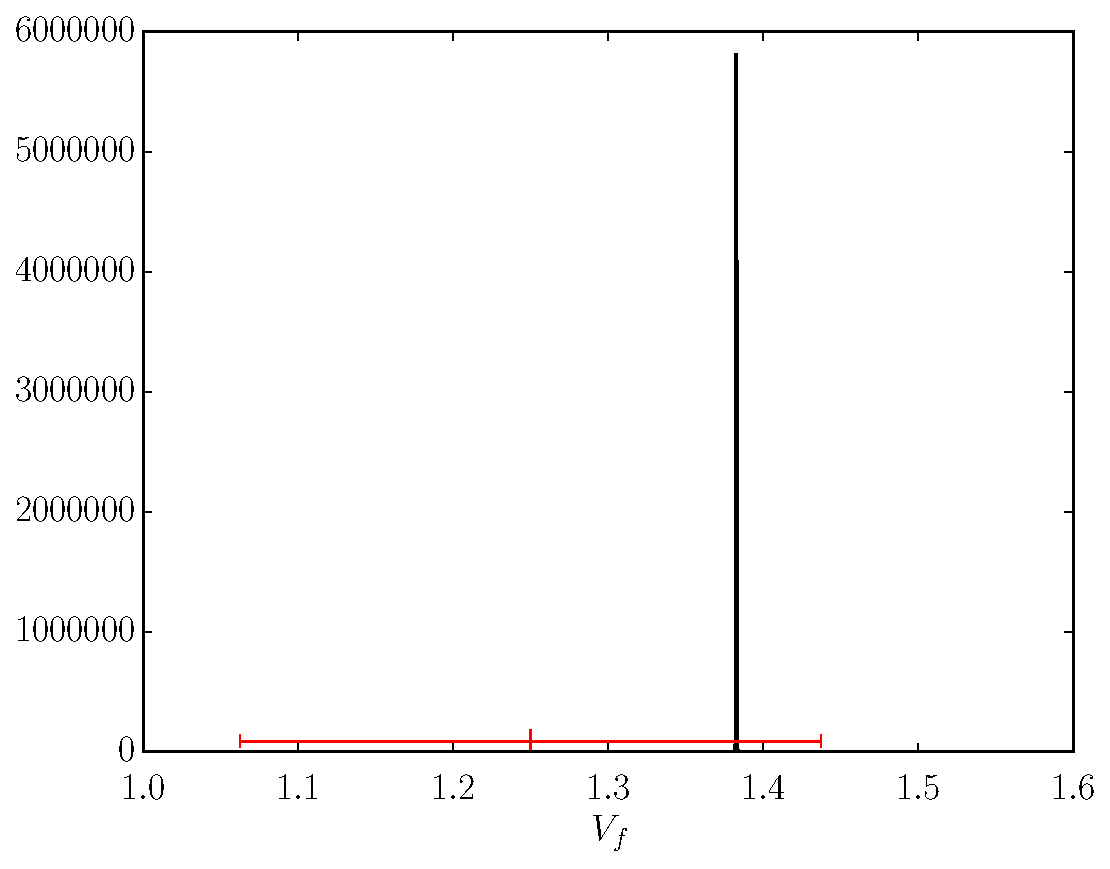
\includegraphics[scale=0.7]{one_parameter/flamespeed_calculation/flame_40.pdf} 
%       }
%     \quad
%\subfloat[Flame speed for 46 \% ozone \label{subfig-1:dummy}]{
%        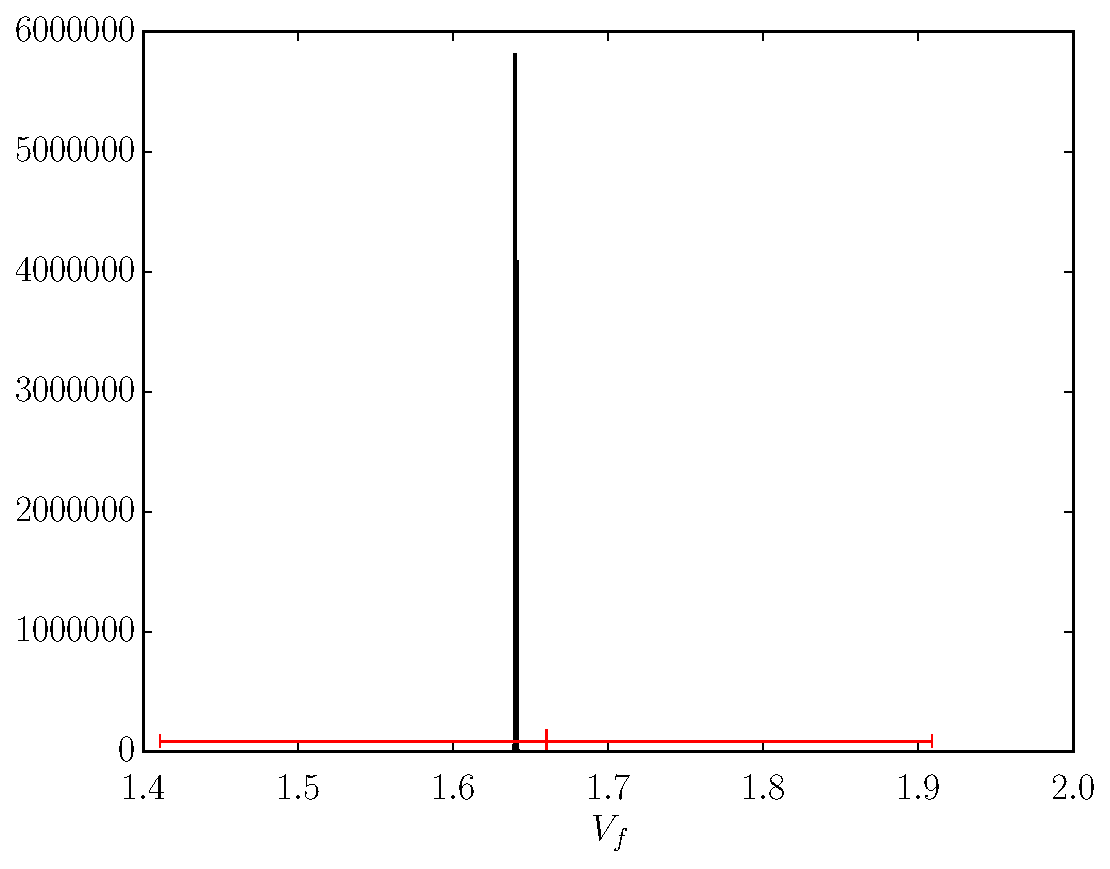
\includegraphics[scale=0.7]{one_parameter/flamespeed_calculation/flame_46.pdf} 
%            }  
%\end{figure}
%
%
% \begin{figure}[H]
%  \ContinuedFloat
%  \centering
%   \subfloat[ Flame speed for 53 \% ozone \label{subfig-1:dummy}]{
%        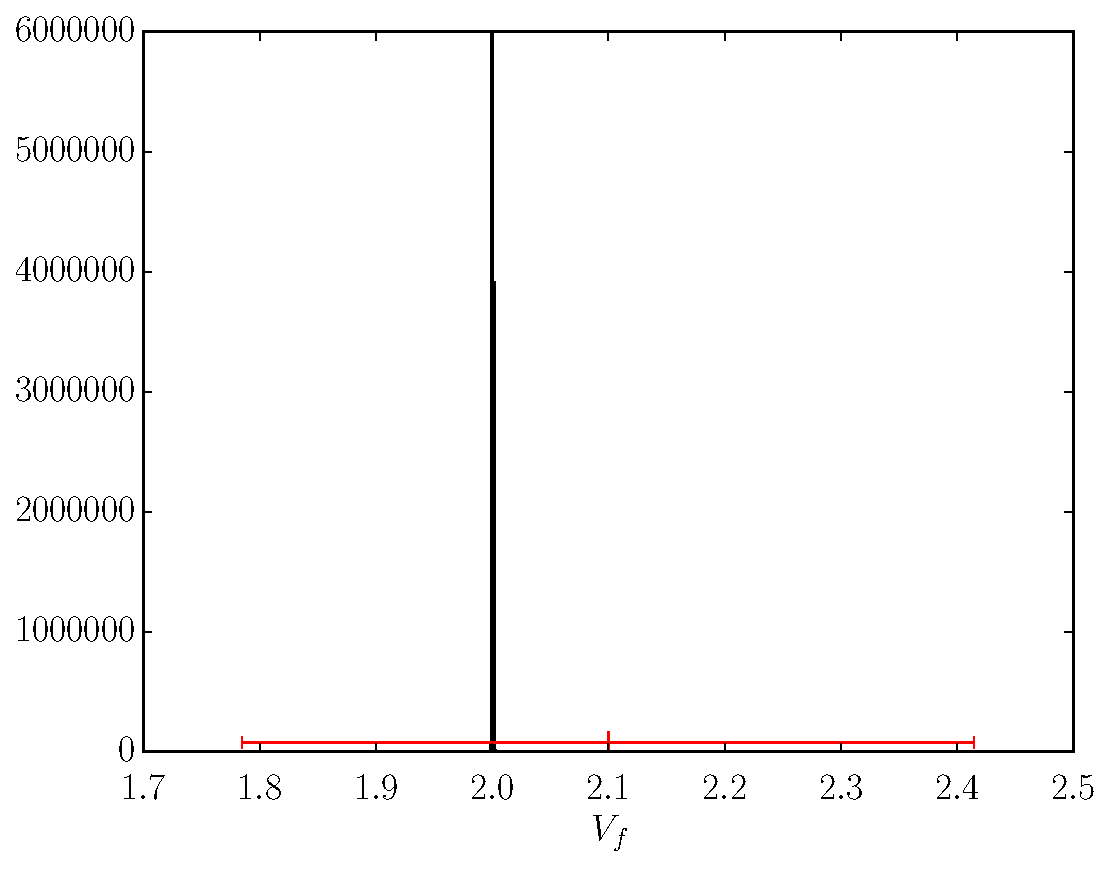
\includegraphics[scale=0.7]{one_parameter/flamespeed_calculation/flame_53.pdf} 
%       }
%     \quad
%\subfloat[Flame speed for 75 \% ozone \label{subfig-1:dummy}]{
%        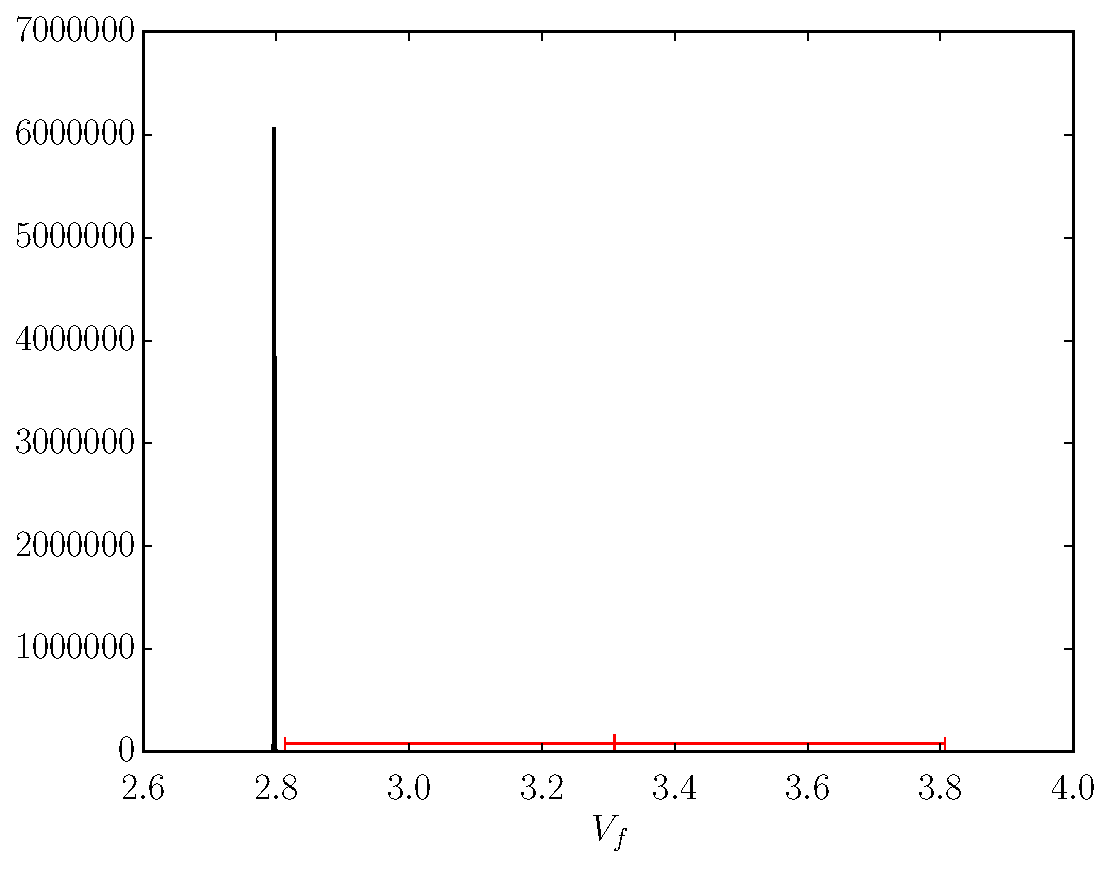
\includegraphics[scale=0.7]{one_parameter/flamespeed_calculation/flame_75.pdf} 
%            }  
%\end{figure}
%
%
% \begin{figure}[H]
%  \ContinuedFloat
%  \centering
%   \subfloat[ Flame speed for 100 \% ozone \label{subfig-1:dummy}]{
%        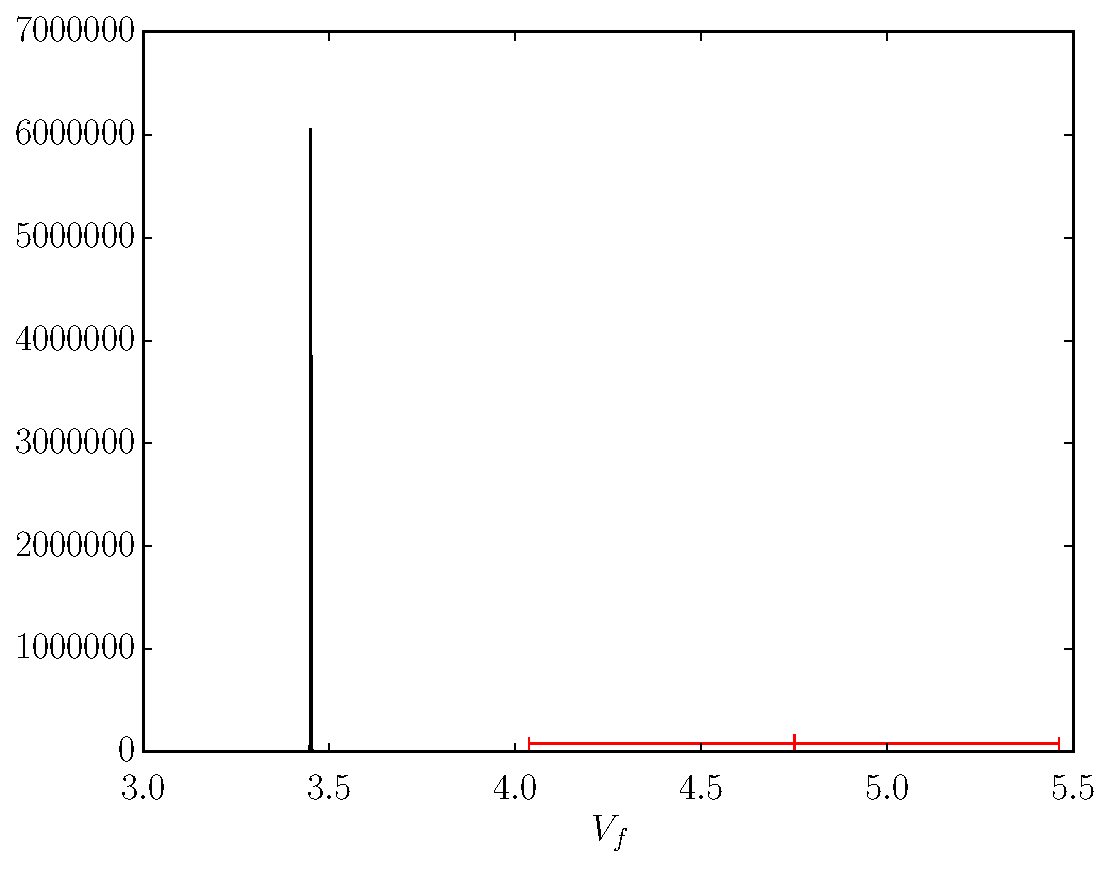
\includegraphics[scale=0.7]{one_parameter/flamespeed_calculation/flame_100.pdf} 
%       }
%  \caption{Flamespeed Data fit}
%\end{figure}